\renewcommand{\taskname}{FUNGHI}
\renewcommand{\timelimit}{1 sekunda}
\renewcommand{\memorylimit}{32 MB}
\renewcommand{\score}{50 bodova}

Nakon što su pojeli sve kolačiće s vještičine kuće, Ivica i Marica naručili su jumbo pizzu. Pizza je uskoro stigla, narezana na osam komada. Ivica i Marica pizzu će podijeliti popola tako da svatko od njih dobije jedan cijeli "polukrug" pizze, tj. četiri uzastopna komada.

Marica jako voli šampinjone i želi ih dobiti što više. Budući da se na nekim komadima pizze nalazi manje, a na nekima više šampinjona, Marica je zamolila Ivicu da pizzu podijele tako da se na njezinim komadima nađe što više šampinjona.

Pomozite Ivici i Marici! Oni će vam reći koliko se šampinjona nalazi na svakom od osam komada pizze, a vi pronađite \textbf{najveći ukupan broj šampinjona koji Marica može dobiti}. Sljedeća slika prikazuje najbolju podjelu za drugi test primjer niže (brojem 1. označen je prvi komad naveden u ulaznim podacima):

\begin{center}
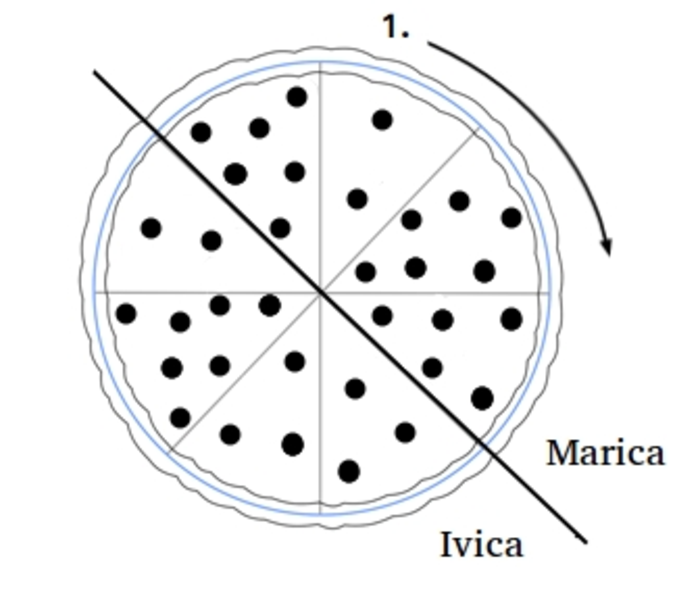
\includegraphics[width=.4\linewidth]{funghi/slika.pdf}
\end{center}

\strut

\naslov{ulazni podaci}

U osam redaka nalazi se po jedan cijeli broj $\check{S}_i$ ($0 \leqslant \check{S}_i \leqslant 50$, $i = 1, 2, \ldots, 8$).
Ovi su brojevi količine šampinjona na komadima pizze, pri čemu su komadi dani redom u smjeru kazaljke na satu.

\strut

\naslov{izlazni podaci}

U jedini redak ispišite traženi broj iz teksta zadatka.

\strut

\naslov{primjeri test podataka}

\begin{center}
\fontfamily{\ttdefault}
\fontsize{10pt}{1em}
\selectfont
\begin{tabu}to 0.99\textwidth{|X[1]|X[1]|}
\hline
& \\ 
\rowfont{\fontsize{10pt}{1em}\bfseries}
ulaz & ulaz \\
\verbatiminput{funghi/funghi.dummy.in.1} & 
\verbatiminput{funghi/funghi.dummy.in.2} \\
\rowfont{\fontsize{10pt}{1em}\bfseries}
izlaz & izlaz \\
\verbatiminput{funghi/funghi.dummy.out.1} & 
\verbatiminput{funghi/funghi.dummy.out.2} \\
\hline
\end{tabu}
\end{center}

{
\fontsize{10pt}{1em}
\selectfont
%\textbf{Pojašnjenje prvog primjera:} pojašnjenje pojašnjenje pojašnjenje \\
%\textbf{Pojašnjenje drugog primjera:} pojašnjenje pojašnjenje pojašnjenje
}